%----------------------------------------------------------------------------------------
%       CHAPTER 3
%----------------------------------------------------------------------------------------

\cleardoublepage

\chapterimage{middle_earth.png} % Chapter heading image

\chapter{Ocean circulation II -- general)}\label{ch:ocean-circulation-II}

\hfill \break

\noindent 'Fake' (idealized) Worlds are a useful tool for developing a general understanding of the primary controls on global climate and  biogeochemical cycles -- and here, ocean circulation. Different model resolutions and continental configurations can be generate and run to test specific hypotheses about the role of different boundary condition to emergent patterns of ocean circulation. This can be done both by modifying the boundary conditions of existing and know circulation states (e.g., modern). Idealized Worlds can also be utilized to create a more generalize understanding of system dynamics as well as serving in a fishing expedition for new and unexpected phenomena and system behaviors.

This Chapter will take you through the generation and exploration (analysis) of idealized Worlds.

%------------------------------------------------
\newpage
%------------------------------------------------

\section*{READ.ME}

You are going to need \textbf{MATLAB}, and then clone some (\textbf{MATLAB}) code ... but onto your local computer (not the GENIE computing cluster). Or instead of cloning, downloading and unpacking the code archive will work just fine.



%------------------------------------------------
\newpage
%------------------------------------------------

\section{Modeling methodology}

\vspace{2mm}


%------------------------------------------------
\subsection{cookiegen overview}

For full details on how to generate your own idealized Worlds, derive configurations from GCM output, or adjust existing configurations -- refer to the Chapter on '\textbf{cookiegen}'.




%------------------------------------------------
\newpage
%------------------------------------------------

\subsection{Analysis strategies}

How do you 'judge' the strength and characteristics of deep-water formation, global overturning, and circulation patterns and strength, in general, or their climate (or biogeochemical) impacts? This is not a trivial question. Often, additional ocean tracers are employed in models to generate a quantitative measure of the age of a parcel of water (mean time since it last saw the surface), of some measure of the efficiency of ventilation, or large-scale transport at the surface or at depth.\footnote{We'll see such tracers employed later in the course.} Or rather involved analysis of ocean physics and transport might be employed.

One starting point is to read some of the literature where the climate properties of various hypothetical worlds have been investigated. Such as:
\vspace{1mm}

\begin{itemize}[noitemsep]
\item \textit{Marshall et al.} [2007] -- 'Mean Climate and Variability of the Atmosphere and Ocean on an Aquaplanet', \textit{Journal of the Atmospheric Sciences} \textbf{64}.
\item \textit{Enderton and Marshall} [2009] -- 'Explorations of Atmosphere--Ocean--Ice Climates on an Aquaplanet and Their Meridional Energy Transports', \textit{Journal of the Atmospheric Sciences}.
\item \textit{Ferreira et al.} [2010] -- 'Localization of Deep Water Formation: Role of Atmospheric Moisture Transport and Geometrical Constraints on Ocean Circulation', \textit{Journal of Climate} \textbf{23}.
\item \textit{Smith et al.} [2006] -- 'Global Climate and Ocean Circulation on an Aquaplanet Ocean–Atmosphere General Circulation Model',  \textit{Journal of Climate} \textbf{19}.
\end{itemize}

\vspace{1mm}
In addition, the sub-sub-sections that follow outline some simple diagnostics and ways of going about some quantitative analysis.

%------------------------------------------------

\subsubsection{Simple/global diagnostics}

\vspace{1pt}
\begin{itemize}[noitemsep]
\vspace{1mm}
\item In the \textbf{biogem} output results folder, there is a time-series file named: \\\textsf{\footnotesize biogem\_series\_misc\_opsi.res} \\This contains a summary of the evolution with time, of the minimum and maximum (anywhere) global overturning stream-function values.
\vspace{1mm}
\item If you have the ventilation age tracer activated, there will also be a time-series output:  \\\textsf{\footnotesize biogem\_series\_misc\_col\_age.res} with fields for: \\\texttt{\small mean global ventilation age (yr) / surface ventilation age (yr) / benthic [> 2000 m] ventilation age (yr)}.
\vspace{1mm}
\item Another simple property of the climate system that you might consider in terms of possible explanations for observed large-scale ocean circulation states, is the pole-to-equator temperature gradient, both in terms of atmospheric temperature, and ocean surface temperature\footnote{\textbf{Panoply} has an option for plotting the zonal mean, from which you could read off pole-to-equator temperature gradients.} (although they should presumably be closely coupled).
\\Why? Because the large scale (overturning) circulation of the ocean should be transporting heat from the high latitude surface to the deep ocean. This presumably would act to reduce latitudinal temperature gradients. In contrast, a strong zonal slow might prevent latitudinal transport of heat.
\\A \textit{time-series output} is provided:  \\\textsf{\footnotesize biogem\_series\_misc\_p2e.res} \\which is the annual average SAT (surface air temperature) gradient between lowest and highest latitudes in the model, averaged over the 2 hemispheres.
\end{itemize}

%------------------------------------------------

\subsubsection{Spatial netCDF fields}

In a physics-only (T + S tracer) configuration of \textbf{cookie} you are  somewhat limited in what you can look at. A good staring point is the previous tutorial on ocean circulation and AMOC stability (in the context of the modern world, climate and continental configuration). For instance, you know already how to plot and visualize the MOC using \textbf{Panoply}. The Atlantic basin and hence the existence of an AMOC, is pretty specific and unique to the modern world, so likely you'll need to focus on the global MOC. (A good starting point is to familiarize yourself with the pattern and intensity of the modern.)

For example -- the \textsf{\footnotesize drakeworld } configuration gives rise to a global MOC pattern as shown in Figure \ref{fig:paleo_drakeworld.opsi}.

This is stored as the variable \textsf{\footnotesize phys\_opsi} in the netCDF file \textsf{\footnotesize fields\_biogem\_2d.nc}. Remember that the first time-slice plotted in \textbf{Panoply} is the first time-slice saved by default :(.

\begin{figure}[H]
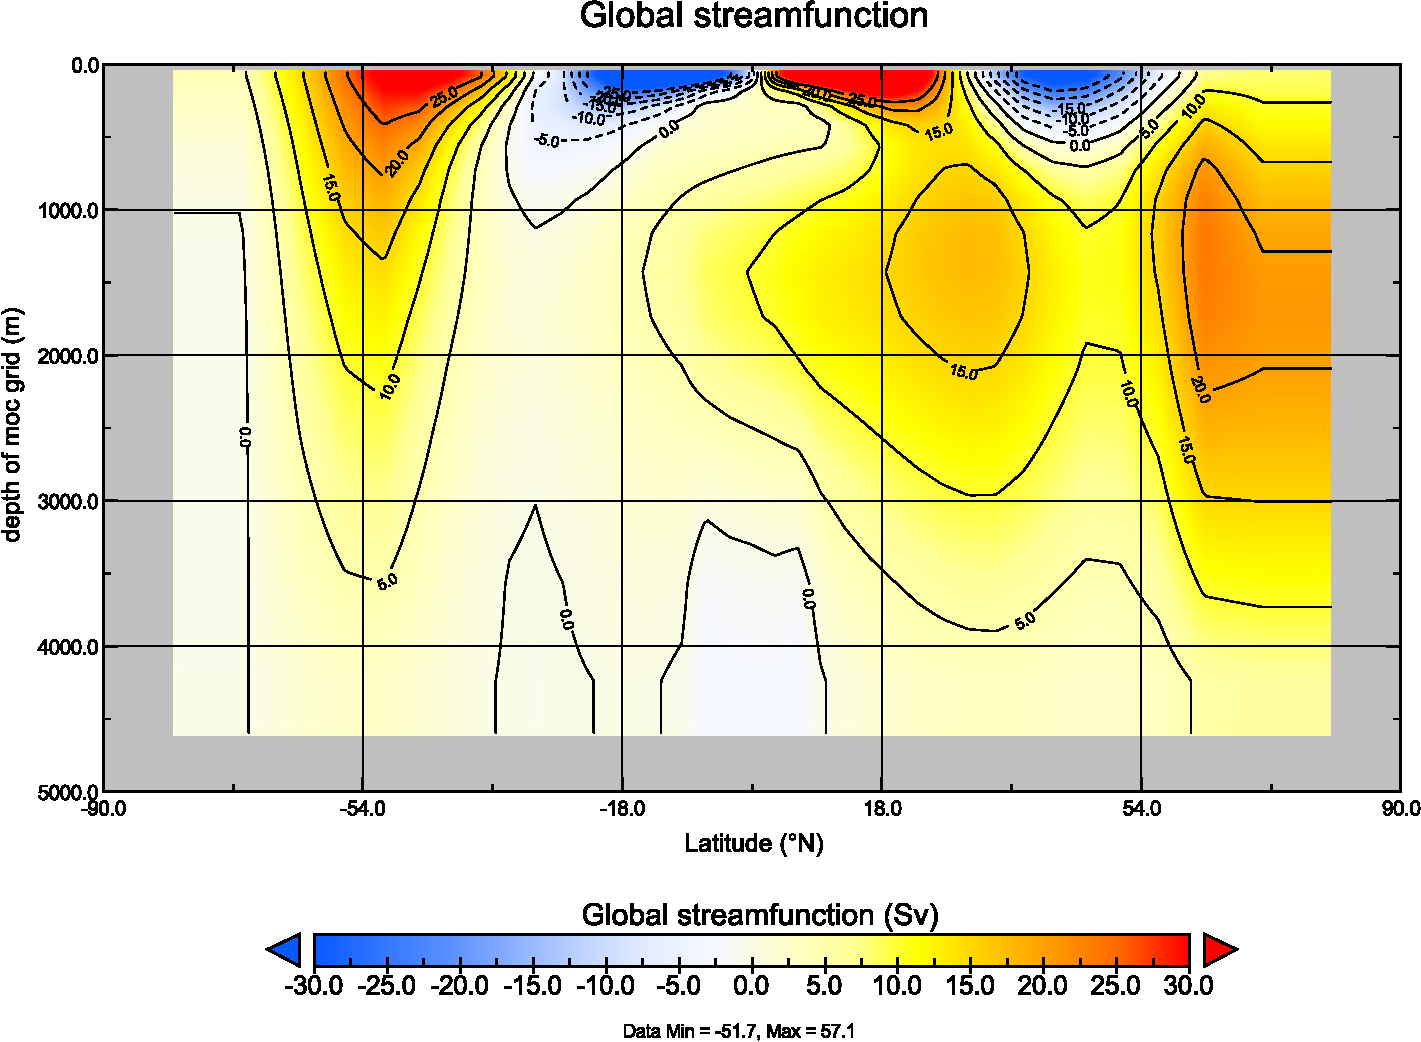
\includegraphics[width=0.6\textwidth]{paleo_drakeworld_opsi.pdf}\centering
\vspace{-0mm}
\caption{Drakework world overturning circulation.}
\label{fig:paleo_drakeworld.opsi}
\end{figure}

You can also plot the barotropic circulation using \textbf{Panoply} -- the variable is called \textsf{\footnotesize phys\_psi} -- this is shown in Figure \ref{fig:paleo_drakeworld.psi}.

\begin{figure}[H]
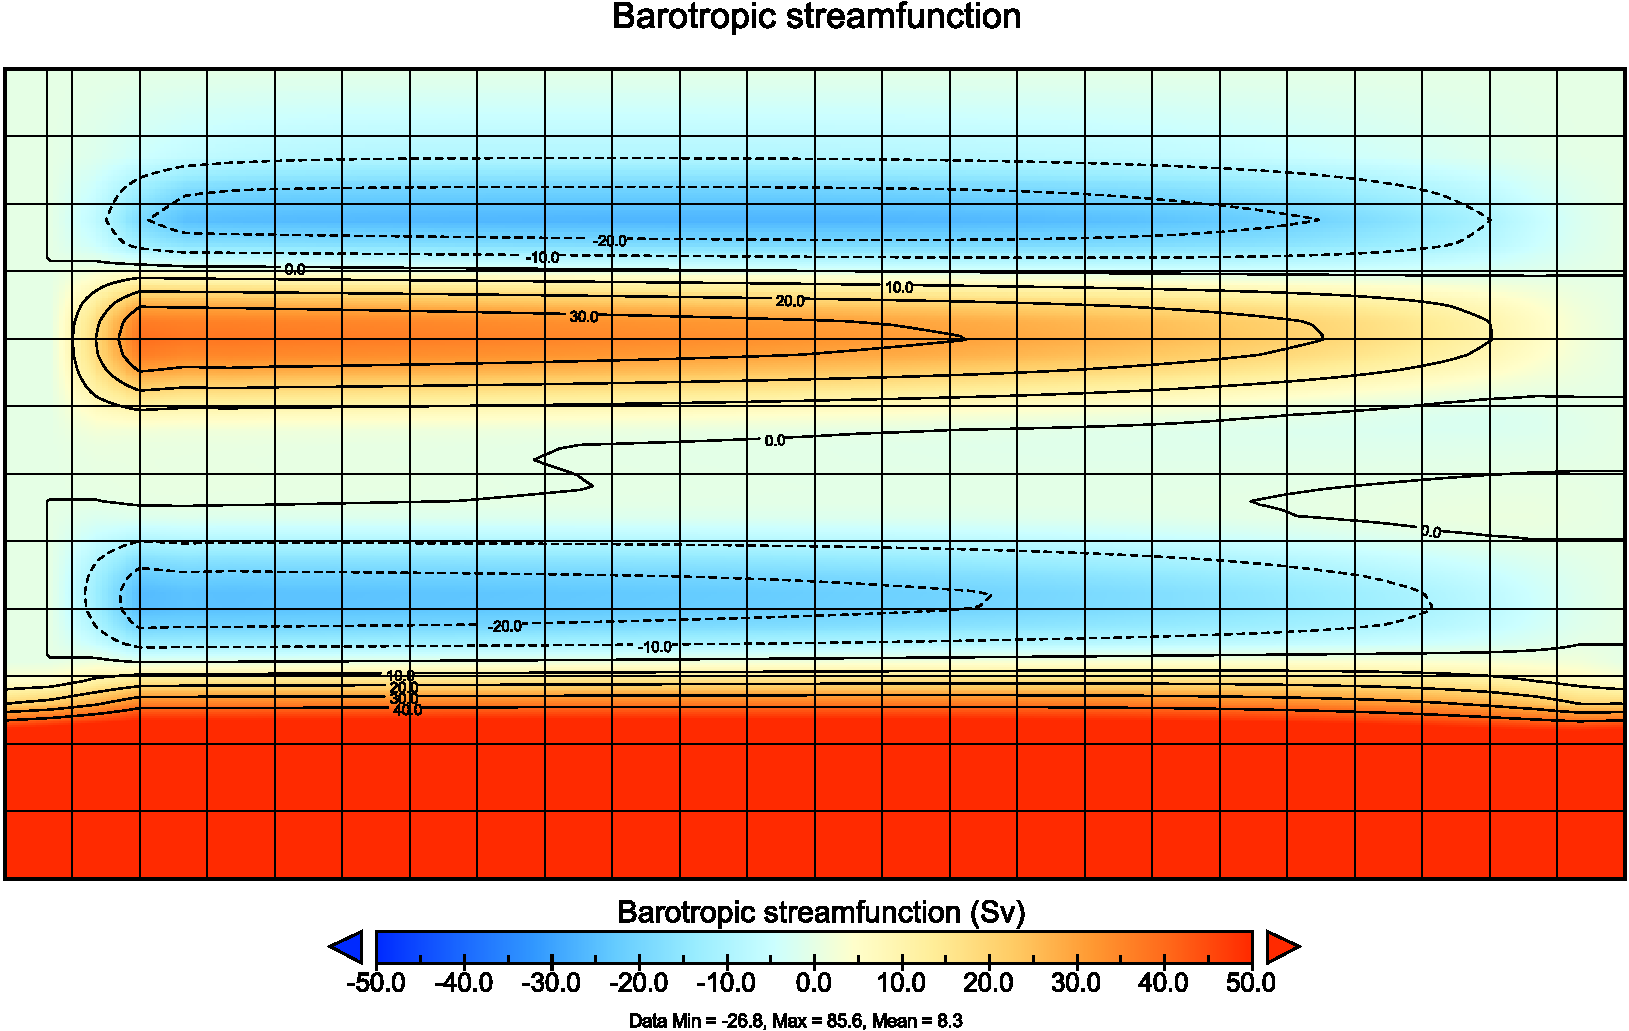
\includegraphics[width=0.5\textwidth]{paleo_drakeworld_psi.pdf}\centering
\vspace{-0mm}
\caption{Drakework world barotropic circulation.}
\label{fig:paleo_drakeworld.psi}
\end{figure}

Finally in \textbf{Panoply}, you might plot the current field (surface or otherwise), as per Figure \ref{fig:paleo_drakeworld.v}.

\begin{figure}
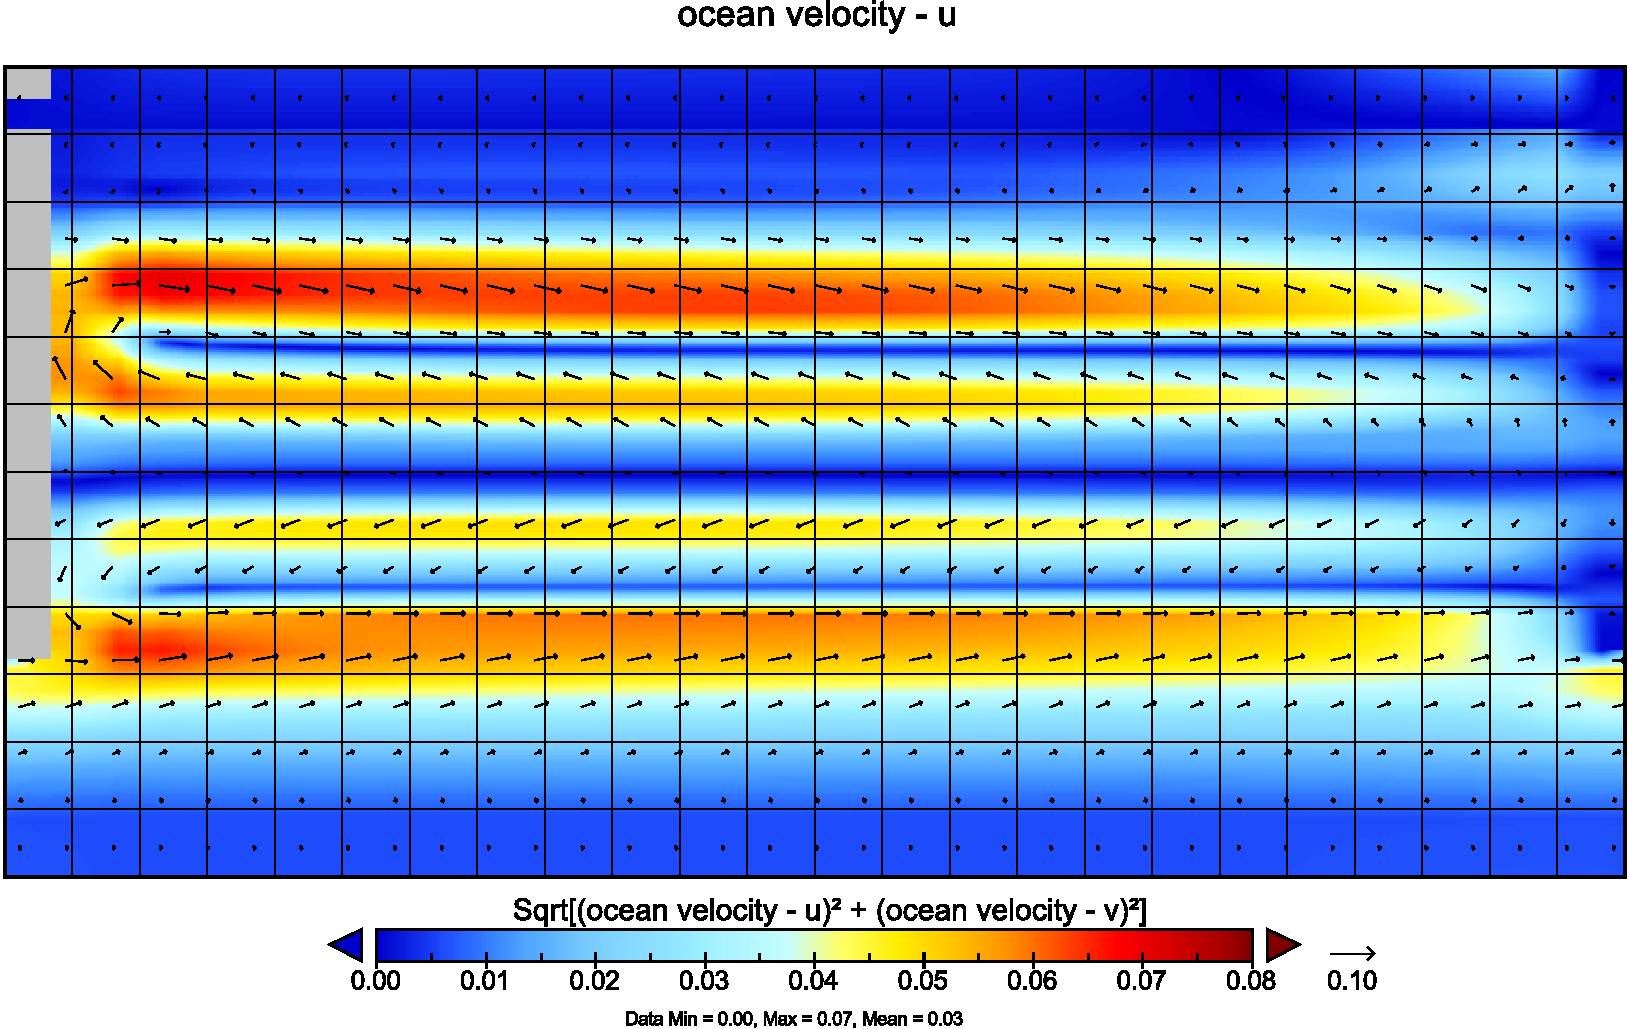
\includegraphics[width=0.5\textwidth]{paleo_drakeworld_v.pdf}\centering
\vspace{-0mm}
\caption{Surface current velocity field (arrows) plus speed (color scale).}
\label{fig:paleo_drakeworld.v}
\end{figure}

%------------------------------------------------
\subsubsection{'Age tracing' of ocean circulation}

Refer to the previous chapter, or the 'HOW-TO' chapter (under: 'Add a water mass age tracer') in the \textbf{cookie} manual.

%------------------------------------------------

\subsubsection{'Color tracing' of ocean circulation}

If you have both 'red' and 'blue' color tracers selected (and a total of 4 ocean tracers compiled into the model), you can use 'red' for ventilation age and 'blue' for color-tracing -- refer to the previous chapter for \textit{user-config} parameter settings, a suitable \textit{forcing}, and further information.

Note that if you only have the 'red' tracer, you can only use this for one of age and color-tracing. To use if for color tracing, ensure that neither of the follow parameter settings are present in your \textit{user-config} file:

\small\vspace{-2pt}\begin{verbatim}
bg_ctrl_force_ocn_age=.true.
\end{verbatim}\vspace{-2pt}\normalsize

and

\small\vspace{-2pt}\begin{verbatim}
bg_ctrl_force_ocn_age1=.true.
\end{verbatim}\vspace{-2pt}\normalsize

OR, that both are set to \texttt{false}. OR that neither parameter appears at all (the default for both is \texttt{\small false}).

%------------------------------------------------
\newpage
%------------------------------------------------
%
\section{Exploring the controls on ocean circulation}

%------------------------------------------------

There are a variety of different ways of visualizing and quantifying ocean circulation and its controls, in \textbf{cookie}.

%------------------------------------------------

\subsection{Model investigation over-view}

In not exploring beyond the modern continental configuration and associated state of large-scale ocean circulation and climate in \textbf{cookie}, you may not come to any particularly general or fundamental insights into ocean circulation controls. In any case, the modern and future (and recent glacial past) ocean circulation states and dynamics have been picked over by 1000s of researchers, writing 100,000s of  publications (although we still do not necessarily fully understand modern/future ocean circulation, let along that at the time of the last glacial).

A broader (or more fun) approach is to generalise the problem and consider fundamentally different configurations of ocean basins and climate. This is what you will be doing. But first, some potted advice:

\vspace{2mm}
\begin{itemize}[noitemsep]
\vspace{1mm}
\item Try and define a hypothesis, or hypotheses, to pursue and test. These need only be very rough at the outset -- you'll likely find that you get new ideas and can either refine your original hypotheses, or come up with new ones, as you start to play with the model and see what is feasible and not feasible in terms of analysis.
\vspace{1mm}
\item Create a plan of study -- what sort of experiments, now many, how are they going to be analysed, how do they all fit together in addressing the overarching hypotheses? Again -- it is very likely that your plan will evolve as you go along, but try and start out with something to guide you rather than wandering randomly in model world ...
\vspace{1mm}
\item For creating and an using different worlds -- write down a list or make a table of the configurations to be explored, why you have chosen them, and then summarize what you are finding. It might be helpful to draw out on paper first the outline of the continental configurations you want, and then create these and run them. (Again, the details of this will very likely evolve.)
\vspace{1mm}
\item Once you have some sort of idea what are are going to do -- plan the experiments. This is important because to run the model to steady state is not trivial. Perhaps plan on having to run the model for 5,000 years\footnote{Even so, you should try running the model much longer to be confident that 5,000 years is OK (and sufficiently close to final equilibrium).} in order to achieve a fully spun up ocean circulation state. You might get away with shorter runs, but know in advance what sort of error this would induce and whether the error might be 'important' (impact your analysis and conclusions)? Once you have a list and know how long each model experiment might take, you can plan out when they will be run on the cluster (presumably on the queue) and when the results will be analysed. Note that it is a virtual certainty that once you have analysed the results of the first set of experiments, you will want something different (and will then need to revise the plana and list of experiments and analysis etc.).
\end{itemize}
\vspace{2mm}

\noindent Overall -- scientific investigations with simplified (and relatively fast) Earth system models tend to become a somewhat iterative undertaking and can involve significant trail-and-error. (This is healthy and to be expected and even enjoyed!) Rarely, can you devise at the outset, a single run or set of experiments, and it turns out this is completely sufficient. If you do not see something you do not understand in the results of the initial model experiments, you are either God (e.g. the Spaghetti Monster or Invisible Pink Unicorn), or not doing it properly. Expect to see things that interest you and lead you off on a tangent (hopefully -- this is how research should be).

Finally -- \uline{remember} that in swapping between different continental configurations (and \textit{base-configs}), \textbf{cookie} currently requires the model executable to be  re-compiled.\footnote{Note that if the \textit{base-config} is the same as the previous experiment, but you have changed a parameter value (in the \textit{user-config}), you do not need to re-compile.} This ... cannot happen on the compute nodes of the cluster if you submit an experiment using a different \textit{base-config}. When changing to a new \textit{base-config}: \uline{first}, run the model briefly interactively (i.e. at the command line). Once it has compiled (and started running), the experiment can be killed (\textsf{ctrl-c}) and now it is good to submit to the queue as a job. In any case, in utilizing a new configuration that you may never have used before, it is good practice to test it first (e.g. watch it run for a short period).

%------------------------------------------------

\subsection{Deep-water formation (\& baroclinic circulation)}

The first investigation is to explore the controls on the strength and large-scale structure of ocean circulation, particularly in terms of the global meridional overturning circulation (MOC), and associated with this -- where the primary sites of deep-water formation are.

There are  2 key controls to this:

\vspace{2mm}
\begin{enumerate}
\item \textbf{Temperature.}
\\This is presumably mostly a function of latitude (i.e. the further North or South, the more suitable the site will tend to be for deep-water formation) and to some extent season. There will also be an influence of the prescribed planetary albedo (which includes the effect of clouds) as well as of sea-ice (if it is present).
\vspace{2mm}
\item \textbf{Salinity.}
\\This will generally be controlled by P-minus-E -- the balance between precipitation to the ocean surface as well as fresh-water run-off form the continents, vs. evaporation from the ocean surface. Sea-ice may also be a key factor, in e.g. leading to the (seasonal) rejection of dense salty brine (and removal of freshwater to the forming ice).
\end{enumerate}
\vspace{2mm}

In turn, this suggests two sets of 'knobs' in the model that can be modified and that may influence the patterns and magnitude of temperature and salinity across the ocean surface:

\vspace{1mm}
\begin{enumerate}
\vspace{1mm}
\item \textbf{Continental Configuration.}
\\The configuration of the continents and ocean basins will dictate the shape and location of the highest latitude ocean regions -- presumably the locations where on average, deep-water formation will occur (and hence forming the downwards/sinking limb of the MOC).
\\The relevant model 'knob' is hence how the position and orientation of continental blocks is configured on the surface of the Earth. This (creating or changing the continental configuration used by \textbf{cookie}) can all done using the \textbf{MATLAB} \textbf{cookiegen} program.
\vspace{1mm}
\item \textbf{Global Climate.}
\\The mean and climate as well as the zonal temperature gradients, together with whether or not sea-ice forms (and how much), will modulate both temperature and salinity patterns at the ocean surface.

%------------------------------------------------
\newpage
%------------------------------------------------
In turn, the model knobs here are primarily:
\vspace{1mm}
\begin{enumerate}
\vspace{1mm}
\item Atmospheric \(pCO_{2}\), or in the absence of an explicit carbon cycle, a prescribed radiative forcing:
\vspace{-2pt}\begin{verbatim}
ea_radfor_scl_co2=1.0
\end{verbatim}\vspace{-2pt}
which here, specifies \(\times1\) \(CO_{2}\) equivalent radiative forcing.
\vspace{1mm}
\item One could also adjust the value of the solar constant (here, given with its modern/present-day default value):
\vspace{-2pt}\begin{verbatim}
ma_genie_solar_constant=1368.0
\end{verbatim}\vspace{-2pt}
which has a subtly different effect form changing \(CO_{2}\) radiative forcing, as radiative forcing has a relatively spatially uniform impact, whereas changing the solar constant has a disproportionate impact towards the Equator (where the incident solar shortwave radiation is the greatest). So changing the solar constant is likely to impact the pole-to-Equator temperature gradient. e.g. see: Lunt, D. J., A. Ridgwell, P. J. Valdes, and A. Seale, Sunshade World.: a fully coupled GCM evaluation of the climatic impacts of geoengineering, GRL 35, L12710, doi:10.1029/2008GL033674 (2008).
\vspace{1mm}
\item One could also adjust the planetary albedo, particularly in respect of looking to modify the pole-to-Equator temperature. In the \textbf{cookiegen} created configurations, there is an explicit 1D file specifying the zonal (with latitude) planetary albedo profile:
\vspace{-2pt}\begin{verbatim}
xxxxxxxx.albd.dat
\end{verbatim}\vspace{-2pt}
where \texttt{xxxxxxxx} is the 8-character name of the \textbf{cookiegen} created World. It would be a simple matter of editing the values in the file (between the range of 0.0 and 1.0, for  perfectly absorbing, and perfectly reflective, respectively).\footnote{Best to make a copy of the original file before you modify it.} \uline{Note that the file data order is North-to-South (going from top to bottom in the file)}.
\end{enumerate}
\end{enumerate}
\vspace{2mm}

%------------------------------------------------

\subsection{Gateways and barotropic flow}

The overarching question in the context of ocean gateways and barotropic flow, is a little harder to define succinctly; it has to do with the details of the degree of alignment (or not) of the prevailing wind (stress)
with  gateways, and the degree to which this give rise to strong zonal ocean flow. A good and obvious modern example is the existence of the Drake Passage, between the northern tip of the Antarctic Peninsular, and the southern tip of Souther America, how this aligns with the prevailing Westerlies in the Southern Hemisphere, and hence the nature and strength of the ACC (Antarctic Circumpolar Current).

So the question naturally arises: how misaligned does a gateway have to be relative to the prevailing wind stress maximum, before the circumpolar (or circum-equatorial) flow ceases. What about having multiple gateways and their relative alignment, including what happens if one gateway is aligned with Westerly wind stress, and a second with Easterly wind stress -- who 'wins')? Also -- what about sill depths? For the Drake Passage, the ocean floor, while tectonically messy, is generally relatively deep. What happens to ocean circulation with a progressively shallow sill depth?

%------------------------------------------------
\newpage
%------------------------------------------------

The 3 key controls in this exercise are then:
\vspace{1mm}

\begin{enumerate}
\vspace{1mm}
\item \textbf{Gateway alignment.}
\\The  alignment (or latitudinal correspondence) of a gateway with the maximum of the zonal wind stress.
\vspace{1mm}
\item \textbf{Gateway width.}
\\The width of a gateway (and how important this is in exerting control on ocean circulation).
\vspace{1mm}
\item \textbf{Sill depth.}
\\The sill depth! This could be uniform in depth across the gateway (easiest/best) or could be varying (probably not so easy to learn anything).
\end{enumerate}
\vspace{2mm}

There are a number of changes that can be made in the model to explore the importance (or not) of the 3 controls listed above:
\vspace{1mm}

\begin{enumerate}
\vspace{1mm}
\item \textbf{Land-sea mask.}
\\The model knob is hence how the width and location of gateways has bene defined in the land-sea mask. There is also the question of how many gateways (and their respective position).
\\As before, this (creating or changing the continental configuration used by \textbf{cookie}) is all done using the \textbf{MATLAB} \textbf{cookiegen} program. Any of the given example \textbf{cookiegen} configurations: \textsf{drakeworld}, \textsf{eqpasworld}, \textsf{ridgeworld}, or \textsf{waterworld}, could be taken as starting points -- copying and renaming the configuration \textsf{.m} file, as well as the \textsf{.dat} file in the \textsf{INPUT} directory.
Or start from scratch and a the 'blank' (initially all ocean) example configuration.\vspace{1mm}
\\Note that a gap between 2 land masses must be \uline{2 or more cells wide}, to count as a gateway and allow barotropic flow in \textbf{cookiegen}).
\vspace{1mm}
\item \textbf{Ocean bathymetry.}
\\The bathymetry (ocean floor depth) can be changed to alter the sill depth. The easiest way to do this is probably within the \textbf{cookiegen} editor, ensuring the following input parameter setting is set:
\vspace{-2pt}\begin{verbatim}
opt_user=true; % [false/true] enable user input to grid
\end{verbatim}\vspace{-2pt}
in the configuration \textsf{.m} file.
\vspace{1mm}
\item \textbf{Wind stress strength.}
\\Although it is messy to attempt to edit the profile of the applied wind-stress field, it is possible to scale its impact on ocean circulation lower and higher. The \textbf{cookie} parameter for this is:
\vspace{-2pt}\begin{verbatim}
go_13=1.531013488769531300
ea_11=1.531013488769531300
\end{verbatim}\vspace{-2pt}
Somewhat bizarrely ... it appears twice ... with different parameter names. Both parameters must be changed to the same value. Place these lines (of the new parameter value assignments) in the \textit{user-config} file for the experiment. Higher values result in a stronger applied wind-stress on the ocean surface.
\vspace{1mm}
\\Note that although this is the simplest change to make, it may not have such a clear scientific question associated with it (other than the obvious and trivial).
\end{enumerate}




%----------------------------------------------------------------------------------------
%----------------------------------------------------------------------------------------